\documentclass{report}
\usepackage{graphicx}
\usepackage{xepersian}
\usepackage{geometry}
\settextfont[Scale=1.2]{XB Zar}
\renewcommand{\baselinestretch}{1.8}

% absolute position title
\usepackage{textpos}

% section numbering
\renewcommand{\thesection}{\arabic{section}}
\renewcommand{\thesubsection}{\thesection.\arabic{subsection}}
\renewcommand{\thesubsubsection}{\thesection.\arabic{subsection}.\arabic{subsubsection}}

\title{
\begin{normalsize}
به نام خدا
\end{normalsize}
\\[4cm]
اصول و مبانی خطایابی نحوی
}
\author{علیرضا نوریان
\\
\\ \small دانشگاه علم و صنعت ایران
\\ \small noorian@comp.iust.ac.ir
}
\begin{document}
\maketitle
%\begin{textblock*}{15cm}(0cm,-9cm)\centering به نام خدا \end{textblock*}

\tableofcontents

\begin{abstract}
نحو\LTRfootnote{Syntax} جمله بسیار با اهمیت و البته خطاپذیر است. در این پژوهش ابتدا تجزیه‌ی نحوی که تقریبا اساس همه‌ی روشهای خطایابی نحوی است، مرور خواهد شد و در ادامه جایگاه خطایابی نحوی و روشهای انجام آن خواهند آمد. در پایان نیز  تعدادی از سامانه‌هایی که برای انجام خطایابی نحوی در زبانهای مخلتف طراحی شده‌اند، با توضیح مختصر، فهرست خواهند شد. لازم به ذکر است که هر آنچه در ادامه می‌آید به نقل از مقالاتی است که قبل از سال 2000 میلادی تالیف شده‌اند.
\\
\\
واژگان کلیدی: خطایابی نحوی، تجزیه‌ی نحوی، پردازش زبان طبیعی

\end{abstract}

\section{مقدمه}
سامانه‌های پردازش زبان طبیعی از کاربر انسانی ورودی می‌گیرند و این ورودی ممکن است دچار خطا باشد. تشخیص این خطاها در سطوح زیر انجام می‌شود \cite{ct2}:
\begin{itemize}
\item
خطایابی لغوی: واژه‌ها (غیر از اسمهای خاص) باید در فرهنگ لغات زبان موجود باشند.
\item
خطایابی نحوی: جمله باید با دستور زبان\LTRfootnote{Grammar} تطابق داشته باشد.
\item
خطایابی معنایی: جمله باید حداقل یک معنی صحیح داشته باشد.
\item
خطایابی کاربردی: جمله باید در بافت\LTRfootnote{Context} معنای صحیح بدهد.
\end{itemize}
همانطور که گفته شد، خطایابی نحوی به معنی بررسی مطابقت میان جمله و دستور زبان است. از این رو تقریبا همه‌ی روشهای تشخیص و اصلاح خطاهای نحوی تلاش می‌کنند جمله را بر اساس دستور زبان تجزیه کنند و عدم موفقیت در تجزیه را به عنوان خطای نحوی گزارش می‌دهند. در طراحی این روشها سعی بر این است که جمله حتی اگر خطا داشته باشد، به درستی تجزیه شود تا خطای جمله دقیقا مشخص شده و قابل اصلاح باشد. در ادامه برای روشن شدن روشهای خطایابی نحوی، تجزیه‌ی نحوی را بررسی می‌کنیم.

\section{تجزیه‌ی نحوی}
تجزیه‌ی نحوی به معنی مشخص کردن نقش دستوری هر واژه در جمله است. حاصل تجزیه‌ی نحوی جمله، درختی مانند درخت نشان داده شده در شکل \ref{parsing} است. ریشه‌ی درخت نشانه‌ی کل جمله و برگهای درخت، واژه‌ها هستند.
\begin{figure}[h]
\centerline{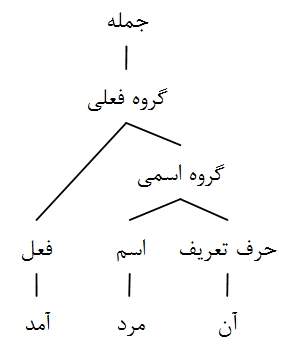
\includegraphics[width=5cm]{tree}}
\caption{\label{parsing} نمونه درخت تجزیه}
\end{figure}
\\
روشهای تجزیه‌ی نحوی برای بسط دادن گره‌ها از دستور زبان استفاده می‌کنند. در \cite{ct2} دو نگاه اصلی در طراحی این الگوریتمها مطرح شده است:

\subsection{تجزیه‌ی بالا به پایین}
در روش بالا به پایین\LTRfootnote{Top-down}، الگوریتم از گره ریشه شروع به کار کرده و با بسط دادن گره‌ها، نوعی جستجو انجام می‌دهد تا به تمام واژه‌های جمله برسد. در این روش هرگز درختهایی که به ریشه نمی‌رسند، بررسی نمی‌شوند. البته بسیاری از درختهایی که با ورودی سازگار نیستند، بررسی می‌شوند.
\subsection{تجزیه‌ی پایین به بالا}
در روش پایین به بالا\LTRfootnote{Bottom-up}، الگوریتم از واژه‌های جمله شروع به کار کرده، سعی می‌کند با اعمال قوانین دستور زبان (‌به طور معکوس‌) به ریشه دست‌ یابد. در این روش تنها، درختهایی که با ورودی سازگارند، بررسی می‌شوند. البته بسیاری از درختهایی که نمی‌توانند به ریشه برسند، بررسی می‌شوند.

برای رفع نقایص دو روش، روشهایی ابداع شده که در آنها از مزایای هر دو استفاده می‌شود. تجزیه‌ی مبتنی بر دستور زبان، تنها برای جمله‌هایی که خطای نحوی ندارند، قابل اعمال است. آنچه در این پژوهش مورد بررسی قرار می‌گیرد، تجزیه‌ی نحوی برای جمله‌هایی است که ممکن است، خطای نحوی داشته باشند.

\subsection{دستور زبان مستقل از متن تقویت شده}
دستور زبان مستقل از متن در بیان قوانین نحوی توان توصیفی و انعطاف‌پذیری پایینی دارد. برای رفع این مشکلات دستور زبان مستقل از متن تقویت شده‌ در بعضی از سامانه‌ها برای تجزیه‌ی نحوی مورد استفاده قرار می‌گیرد. در این دستور زبان هر متغیر تعدادی ویژگی دارد و هرکدام از این ویژگی‌ها می‌تواند مجموعه‌ای از مقادیر را بپذیرد \cite{ct4}. 
برای نمونه عبارت اسمی «این کتابها» با استفاده از قانون (بسیار ساده شده‌ی)
<گروه اسمی (تعداد)> $\Longleftarrow$ <حرف تعریف> <اسم (تعداد)>
که جزئی از یک دستور زبان مستقل از متن تقویت شده است، به عنوان یک گروه اسمی جمع پذیرفته می‌شود. اما برای پذیرفتن همین عبارت با استفاده از دستور زبان مستقل از متن باید از قانون 
<گروه اسمی جمع> $\Longleftarrow$ <حرف تعریف> <اسم جمع>
استفاده کرد. در واقع یک قانون در دستور زبان مستقل از متن تقویت شده، معادل مجموعه‌ای از قوانین در دستور زبان مستقل از متن است. 

\subsection{قوانین تعدیل شده}
از نظر دستور زبان، جملاتی که خطای نحوی دارند، جز‌ء زبان محسوب نمی‌شوند. بعضی از تجزیه‌گرها با استفاده از قوانین تعدیل شده\LTRfootnote{Relaxed Constraints}، این جملات را تجزیه می‌کنند. برای نمونه در \cite{ct5}، تعدیل قوانین در شبکه‌ی انتقالی تقویت شده\LTRfootnote{Augmented Transition Network (ATN)}، بررسی شده است. هنگامی که روند تجزیه‌ی جمله در یک گره از این نوع شبکه متوقف شود و یالی برای پیمایش وجود نداشته باشد، یکی از یالها که قابلیت اعمال تعدیل را داشته باشد، تعدیل شده و روند تجزیه ادامه می‌یابد. در ادامه شبکه‌ی انتقالی تقویت شده بیشتر معرفی خواهد شد.

ساده‌ترین شکل تعدیل یک قانون، نادیده‌ گرفتن یکی از ویژگی‌هایی است که یک واژه باید داشته باشد تا در نقش خاصی در جمله قرار گیرد. مثلا یک واژه برای اینکه در جمله‌ای برچسب اسم دریافت کند باید به شکل مفرد باشد، ولی قانون تعدیل شده به واژ‌ه‌ی جمع نیز اجازه می‌دهد که این برچسب را دریافت کند. در این نوع تعدیل، در هنگام تعریف قوانین باید مشخص کنیم که شرطهای این قانون چگونه تعدیل می‌شوند.

در تعدیل یک قانون بعضی از شرطها نقیض می‌شوند و برای بقیه‌ی شرطها نیز در هنگام تعریف قانون باید شکل جایگزین در هنگام تعدیل، مشخص شود. یک قانون، ممکن است چند شرط داشته باشد و یا یک شرط به چند شکل تعدیل شود. در این صورت همه‌ی شکلهای مختلف تعدیل قانون اجرا می‌شوند و روند تجزیه با هر کدام از آنها ادامه می‌یابد. برای تعریف نحوه‌ی تعدیل قانون در \cite{ct5} روش دیگری نیز ارائه شده است که مطابق آن یک ساختار سلسله مراتبی میان نقشها تعریف شده و روابط تعدیل قانون در میان نقشها با توجه به ساختار، تعریف می‌شود. 


\section{خطایابی نحوی}
\subsection{ضرورت خطایابی نحوی}
تشخیص و اصلاح خطاهای نحوی در جملات موجب روان شدن متن و تسهیل انتقال مفاهیم توسط آن می‌شود. علاوه بر این، لازمه‌ی فهم یک جمله توسط ماشین، تجزیه کردن آن است. جملاتی که دچار خطای نحوی هستند، با توجه به دستور زبان جزء جملات زبان محسوب نمی‌شوند. بعضی از روشهای خطایابی نحوی مانند روش شبکه محور و روش نمودار محور، در ابتدا سعی می‌کنند جمله را (اگرچه خطا داشته باشد) تجزیه کنند.

\subsection{انواع خطاهای نحوی}
همانطور که اشاره شد، در خطاهای نحوی، قانونی که در جمله رعایت نشده، بخشی از دستور زبان است. این پژوهش، خطایابی نحوی را مورد بررسی قرار می‌دهد و به جزئیات خطاهای نحوی نمی‌پردازد. در \cite{ct3} خطاهای نحوی به طور کلی به دو گروه زیر تقسیم شده‌اند:
\begin{itemize}
\item
خطاهای غیر ساختاری مانند عدم تطابق میان اجزای جمله از نظر شخص، جنسیت و یا تعداد. مثل جمله‌ی «من به مدرسه رفت» که در آن میان فعل و فاعل تطابق وجود ندارد.
\item
خطاهای ساختاری مانند خطا در ترتیب قرارگیری واژه‌ها. مثل جمله‌ی «رفتم من به مدرسه» که در آن جای نهاد و گزاره عوض شده است.
\end{itemize}

\subsection{مراحل تشخیص و اصلاح خطا}
در \cite{ct6} مراحل تشخیص و اصلاح خطا به صورت زیر تقسیم‌بندی شده‌اند:
\begin{itemize}
\item
آشکار‌سازی، مشخص کردن بخشهایی از جمله که احتمالا دچار خطا هستند؛ مانند گروه اسمی
\item
شناسایی، مشخص کردن قوانینی که احتمالا نقض شده‌اند. مانند تطابق میان فعل و فاعل از نظر تعداد
\item
عیب‌یابی، مشخص کردن دلایل احتمالی نقض شدن قوانین. مانند اسم مفرد، به جای اسم جمع
\item
اصلاح، این مرحله در سه بخش انجام می‌شود:
\begin{itemize}
\item
ایجاد گزینه‌های جایگزین برای بخش غلط
\item
مرتب کردن گزینه‌ها بر اساس احتمال آنها
\item
جایگزین کردن محتمل‌ترین گزینه
\end{itemize}
\end{itemize}

\section{روشهای تشخیص و اصلاح خطا}
\subsection{بدون تجزیه‌ی متن}
استفاده از مدل چند‌نگاشت\LTRfootnote{N-Gram} در خطایابی نحوی نارسایی‌های بسیاری دارد \cite{ct7}. جایگزین این مدل، مدلهایی هستند که متن را تجزیه نمی‌کنند و فقط از برچسبهای نحوی\LTRfootnote{Tag} واژه‌ها استفاده می‌کنند. این روشها دقت پایین و سرعت بالایی دارند \cite{ct8}. ارزش‌گذاری جایگزینهای تولید شده برای یک جمله‌ی اشتباه، حداقل کاربرد این روشها است. در ادامه به تعدادی از این روشها اشاره می‌شود:
\begin{itemize}
\item
جستجوی‌ خطا در برچسبهایی که با احتمال خیلی کمی نسبت داده شده‌اند.
\item
جستجوی خطا در نقطه‌ی کمینه‌ی موضعی\LTRfootnote{Local Minimum}، یعنی واژه‌ای که احتمال خیلی کمتری نسبت به واژه‌های اطرافش دارد.
\item
جستجوی خطا در میان جفت واژه‌های متوالی با استفاده از مفهوم احتمال خطا برای هر جفت برچسب که همان نسبت تعداد نمونه‌های اشتباه از آن جفت به تعداد نمونه‌های درست از آن در پیکره‌ی متنی است.
\item
استفاده از برچسب خطا:

در این روش در پیکره برای هر واژه علاوه بر برچسبهایی که می‌تواند بپذیرد، برچسبهایی که اشتباه پذیرفته نیز ثبت می‌شوند. سامانه‌ای که برچسب می‌زند علاوه بر برچسبهای صحیح از برچسبهای خطا هم استفاده می‌کند. اگر واژه‌ای با برچسب خطا، مشخص شد؛ باید اصلاح شود. برای اصلاح می‌توان شکلهای دیگر کلمه را در متن زمینه آزمود و واژه‌ی مناسب را انتخاب کرد.
\end{itemize}

\subsection{روش نمودار محور}
در روش نمودار محور\LTRfootnote{Chart-Based} ابتدا یک تجزیه‌گر پایین به بالا، متن را تجزیه می‌کند. موفق نشدن این تجزیه‌گر در تجزیه‌ی همه‌ی جمله، نشانه‌ی وجود خطا در جمله است. در این موقع یک تجزیه‌گر بالا به پایین شروع به کار می‌کند. این تجزیه‌گر، تعدادی خطای از پیش تعیین شده را برای جمله فرض می‌کند و با این فرض جمله را اصلاح می‌کند. این روش در صورت وجود چند خطا بسیار ناموفق است \cite{ct9}.

در روش نمودار محور، جمله بخش بخش می‌شود و نقش هر بخش با کمک دستور زبان تعیین می‌شود. هر بخش از ابتدای یک واژه شروع شده، تا انتهای همان واژه و یا واژه‌ی دیگری ادامه می‌یابد. با توجه به قوانین از پیش تعیین شده، یکی از نقشهای ممکن برای بخش و در نتیجه تعدادی شرط برای دیگر اجزای جمله فرض می‌شود. به این ترتیب یک درخت جستجو تشکیل می‌شود که رسیدن به برگ در آن به معنی برقراری همه‌ی فرضها در طول مسیر از ریشه تا برگ و تجزیه‌ی کل جمله است. در این درخت می‌توان به روشهای گوناگون جستجو کرد که در \cite{ct10} از روش A* استفاده شده است.

سامانه‌ی CHAPTER \cite{ct11} نیز که از دستور زبان مستقل از متن تقویت شده بهره می‌برد، یک نمونه‌ی دیگر استفاده‌ از روش نمودار محور برای خطایابی نحوی است. مراحل انجام خطایابی نحوی این سامانه در \cite{ct12} شرح داده شده است که در سه مرحله خلاصه می‌شود:

\subsubsection{پیش‌بینی بالا به پایین}
در این مرحله ابتدا یک هدف اولیه تولید می‌شود، که همان خواسته‌ی اصلی مبنی بر تجزیه‌ی کل جمله است. سپس این هدف با استفاده از دستور زبان بسط داده می‌شود. بسط هدف موجب تولید تعدادی ارتباط نیازمندی\LTRfootnote{Need-Arc} بین هدف و زیر هدفهایش می‌شود. هر هدف، فرض کردن برچسبی برای بخشی از جمله است. با نزدیک شدن به برگها، بخشها کوچک و کوچکتر می‌شوند، تا جایی که به هر واژه برچسبی نسبت داده شود. در این مرحله از قوانین تعدیل‌شده استفاده می‌شود، تا اگر جمله خطا هم داشته باشد، قابل تجزیه باشد.

\subsubsection{انطباق پایین به بالا}
پس از بسط دادن هر هدف، یک مرحله انطباق میان زیر‌هدفها و واژه‌های جمله انجام می‌شود. در این مرحله نحوه‌ی محقق شدن نیازمندیها (طی شدن فاصله‌ی میان برچسبها و واژه‌ها) تعیین می‌شود. پس از این مرحله هدف جدیدی تولید می‌شود که زیرهدفی برای هدف قبلی محسوب می‌شود و می‌توان گفت که به واژه‌های جمله نزدیکتر است.

\subsubsection{فرایند تولید مجدد اجزا}
پس از پیش‌بینی و انطباق در صورت وجود خطا در هر کدام از مراحل که به معنی موفق نبودن آنها است، یک خطای محلی تشخیص داده می‌شود و پس از اصلاح خطا، حلقه‌ی پیش‌بینی و انطباق ادامه می‌یابد.

سامانه برای انتخاب میان اصلاحهای ممکن برای یک خطا، به گزینه‌های مختلف امتیاز می‌دهد. برای امتیازدهی معیارهای زیادی وجود دارد. معیارهای ساده‌تر به دستور زبان وابستگی ندارند، مانند فاصله‌ی میان حرفهای واژه‌ی اصلی و واژه‌ی اصلاح‌شده. البته معیارهای پیچیده‌تری هم وجود دارد که به دستور زبان وابسته‌اند، مانند نوع عملی که برای اصلاح لازم است و یا نقش واژه‌ای که مورد اصلاح قرار می‌گیرد. با توجه به معیار نوع عمل، جایگزینی یک واژه بر حذف یا افزودن واژه اولیت دارد.

\subsection{روش شبکه محور}
این روش بر تعدادی قانون از پیش تعیین شده، بنا شده است. هر قانون با فرض وجود یک نوع خطا آن را اصلاح می‌کند. یک قانون به شکل زیر تعریف می‌شود:

\begin{equation}
C_{1}\&C_{2}\&...\&C_{n}\Rightarrow A_{1},A_{2},...,A_{m}
\end{equation}

در این قانون اگر همه‌ی شرطهای $C_{1}$ تا $C_{n}$ برقرار باشند، اعمال $A_{1}$ تا $A_{m}$ به ترتیب انجام می‌شوند. قوانین می‌توانند توسط انسان تهیه و یا با استفاده از یادگیری خودکار\LTRfootnote{Machine Learning}، آموخته شوند.

در این روش ابتدا رویه‌ی تجزیه انجام می‌شود. اگر تجزیه‌ی جمله موفق نبود، یکی از قوانین ممکن اعمال می‌شود و پس از آن دوباره برای تجزیه‌ی جمله اقدام می‌شود. این حلقه تا جایی ادامه می‌یابد که جمله به طور کامل تجزیه شود. چون همیشه چند قانون ممکن برای اعمال در هر مرحله وجود دارد، حاصل این روش، درختی است که در برگهای آن حالتهای مختلف اصلاح جمله به دست آمده است. محتمل‌ترین شکل اصلاح جمله با روش امتیازدهی انتخاب می‌شود.

در \cite{ct13} از شبکه‌ی انتقالی تقویت شده که روشی شبکه محور است، برای اصلاح خطاهای لغوی، نحوی، معنایی و کاربردی استفاده شده است. شبکه‌ی انتقالی تقویت شده ابزاری برای بیان دستور زبان است. این نوع شبکه به گونه‌ای مفهوم فراخوانی تابع را به ماشین متناهی آورده است. برای تجزیه‌ی متن با استفاده از این نوع شبکه، روشهای موجود برای دیگر شکلهای بیان قوانین، نیاز به تغییراتی دارد \cite{ct14}.

در \cite{ct1} ادعا شده که این شبکه‌ها انعطاف‌پذیری لازم برای اعمال قوانین معنایی ندارند. همچنین انجام جستجو برای رسیدن به پاسخ در این نوع شبکه نیاز به نگهداری اطلاعات زیادی در هر گره دارد. یکی از راه‌های رفع مشکلات این روش، تغییر پویای شبکه به طور موقتی است. این راه عملکرد خوبی دارد ولی فرایند آن پیچیده و سرعت آن پایین است.

روش شبکه‌محور تنها مربوط به اصلاح خطا نیست. در مرحله‌ی تجزیه‌ی نحوی که تجزیه‌های مختلفی برای یک عبارت پیشنهاد می‌شود نیز می‌توان از این روش استفاده کرد. برای مثال در سامانه‌ی KURD \cite{ct15} از این روش برای تجزیه‌ی نحوی و بررسی سبکی\LTRfootnote{Style Checking} استفاده شده است. البته در این سامانه مجموعه‌ای از قوانین به ترتیب اعمال می‌شوند و شبکه‌ای از قوانین تعریف نشده است.

\subsection{روش تطابق الگو}
در این روش تعدادی الگوی از پیش تعیین شده، با جمله تطابق داده می‌شوند و بهترین الگو، به عنوان الگوی جمله انتخاب می‌شود. به دلیل امکان وجود خطا در جمله، الگوهایی که تا حدی با جمله تطابق دارند، نیز در امتیازدهی بررسی می‌شوند \cite{ct16}. عبارت 
«\}چنین\{ <گروه اسمی> (مانند | مثل | همچون | چون) \}< گروه اسمی>،\{* \}و|یا\{ <گروه اسمی>»
نمونه‌ی یک الگوی گروه اسمی است. «شاعرانی مانند حافظ» یک نمونه از گروه‌های اسمی است که با این الگو تطابق دارند.

روش تطابق الگو برای اصلاح خطا از روش شبکه محور بهتر است و امکان جستجوی بهتری را فراهم می‌کند. در این روش جایگزین کردن الگوهای نحوی با الگوهای معنایی، موجب تشخیص خطاهای معنایی می‌شود. البته خطا در ترتیب قرارگیری واژه‌ها در این روش به راحتی قابل تشخیص نیست \cite{ct1}.

روش تطابق الگو می‌تواند برای تسریع تجزیه‌ی جمله، در روشهای دیگر نیز به کارگیری شود، برای نمونه:
\begin{itemize}
\item
با تعریف الگوهای صحیح جمله، می‌توان جملاتی را که خطای نحوی ندارد مشخص کرد، تا لزومی به تجزیه‌ی کامل آنها با استفاده از قوانین تعدیل‌شده، نباشد. 
\item
با تعریف الگوهای خطا، می‌توان تعدادی از خطاها را تشخیص داد.
\item
با تعریف الگوهای کلی جمله‌ (که جزئیات زیادی ندارد) می‌توان جمله را به گروه‌واژه‌های مستقل از هم شکست و هر کدام را جداگانه تجزیه‌ی کامل کرد.
\end{itemize}
این ترفندها سرعت تجزیه را بسیار بالا می‌برند، اگرچه وابستگی زیادی به زبان دارند. البته در مواردی هم موجب اشتباه در تجزیه می‌شوند \cite{ct16}.

\subsection{روش مبتنی بر موجودیت}
مفهوم موجودیت\LTRfootnote{Entity} چیزی شبیه برچسب نحوی و البته بسیار خاص‌تر از آن است. در این روش موجودیتهایی که ممکن است در تعامل با سامانه استفاده شوند، کاملا برای آن تعریف می‌شوند. همین باعث می‌شود که سامانه بسیار محدود ولی در عوض بسیار قدرتمند شود. برای مثال در پیاده‌سازی یک سامانه‌ی انتخاب واحد دانشگاه که با زبان طبیعی با کاربر تعامل می‌کند، تمام مفاهیمی که کاربر از آنها استفاده می‌کند (شامل درس، واحد، حذف کردن، اضافه کردن و ...)  به عنوان موجودیت در سامانه تعریف می‌شوند \cite{ct1}.

\subsection{روش یادگیری}
یادگیری، می‌تواند در استخراج قوانین از پیکره بسیار کارآمد باشد. اما برای اصلاح خطا هم می‌توان تنها با استفاده از یادگیری روندی را طراحی کرد. برای مثال در \cite{ct17} از درخت تصمیم‌گیری برای یادگیری نحوه‌ی استفاده از حرفهای تعریف در زبان انگلیسی استفاده شده است.

\subsection{استفاده از چند روش}
روشهای گفته شده می‌توانند به صورت ترکیبی هم مورد استفاده قرار گیرند. سامانه‌ی DYPAR یک نمونه‌ی موفق این روش است. این سامانه متناسب با ورودی از شیوه‌های تطابق الگو، تفسیر معنایی، و تبدیل نحوی برای تجزیه‌ی جمله استفاده می‌کند \cite{ct1}. تفسیر معنایی با استفاده از یک دستور زبان مستقل از متن معنایی و به منظور طبقه‌بندی واژه‌ها و عبارات انجام می‌شود. تبدیل نحوی با استفاده از الگوهای از پیش تعیین شده و به منظور تبدیل عبارت به شکل معادل استاندارد انجام می‌شود \cite{ct18}.

\section{بررسی سامانه‌های طراحی شده}
سامانه‌های متعددی در زبانهای گوناگون برای خطایابی نحوی طراحی شده است. در ادامه بعضی از این سامانه‌ها به طور مختصر معرفی می‌شوند. معرفی سامانه‌ها، موجب می‌شود جنبه‌های پیاده سازی و ابتکارات هر سامانه هم مورد بررسی قرار گیرد. 

\subsection{زبان انگلیسی}
در زبان انگلیسی سامانه‌های زیادی برای اصلاح متن از جهات مختلف ایجاد شده است. سامانه‌ی NOMAD \cite{ct19} یکی از سامانه‌های اولیه در این زمینه و مبتنی بر انتظارات\LTRfootnote{Expectations} است. این سامانه به لحاظ لغوی، نحوی و معنایی متن را بررسی و اصلاح می‌کند. سامانه متن را از چپ به راست می‌خواند و با دیدن هر واژه فرضهایی در مورد معنی و نقش اجزای قبل و بعد از آن واژه در نظر می‌گیرد. در واقع سامانه انتظار دارد با توجه به این واژه، دیگر واژه‌های جمله ویژگی‌های خاصی داشته باشند. تناقض میان فرضهای مورد انتظار حاصل از واژه‌های مختلف، به عنوان خطا ثبت می‌شود. این سامانه تعدادی خطای مشخص را تعیین کرده و هر کدام را به شکلی اصلاح می‌کند. همچنین برای تصمیم‌گیری نهایی در این سامانه از انتخاب کاربر نیز استفاده می‌شود.

\subsection{زبان هلندی}
در یکی از سامانه‌هایی که برای زبان هلندی طراحی شده \cite{ct14}، ابتدا همه‌ی واژه‌ها بررسی و در صورت لزوم اصلاح لغوی می‌شوند. سپس یک واحد پیش‌پردازنده واژه‌ها را ترکیب می‌کند و شبکه‌ای از گروه‌واژه‌ها تشکیل می‌دهد. اگر یکی از واژه‌ها خطا داشته باشد، شبکه‌ی مشابهی برای آن تولید می‌شود که واژه‌ی اصلاح شده در آن قرار دارد. سپس یک تجزیه‌گر نحوی این شبکه را تجزیه می‌کند. اگر جمله خطا داشته باشد، یک اصلاح‌گر نحوی بین اصلاح‌های ممکن محتمل‌ترین را انتخاب می‌کند.

در مرحله‌ی بررسی واژه‌ها، با استفاده از روشهایی مثل در نظر گرفتن واژه‌هایی که با حروف بزرگ شروع می‌شوند به عنوان اسم خاص و‌ در نظر گرفتن واژه‌های ناشناخته که بسیار تکرار شده‌اند به عنوان واژه‌ی اختراعی، واژه‌های ناشناخته تعیین نقش می‌شوند و به مجموعه واژه‌های شناسایی شده اضافه می‌شوند و حتی بروز خطا در آنها هم اصلاح می‌شود. هنگامی که یک واژه مکرراً اشتباه نوشته شده باشد، سامانه دچار اشتباه می‌شود و به همین دلیل پس از اتمام پردازش فهرست این موارد را به کاربر نشان می‌دهد.

از ابتکارات دیگر این سامانه انجام یک نوع اصلاح بسیار سطحی در واحد پیش‌پردازنده است که موجب افزایش سرعت می‌شود. استفاده از شبکه‌ی گروه‌واژه‌ها، تحلیل اصطلاحات و اصلاح تکرار بیجای واژه را آسان می‌کند. در این سامانه از دستور زبان مستقل از متن تقویت شده استفاده می‌شود. 

\subsection{زبان فرانسه}
در سامانه‌ی ADS \cite{ct7} که برای تبدیل گفتار به متن طراحی شده، در مرحله تبدیل صدا به متن، جملاتی پیشنهاد می‌شوند. سپس یک تجزیه‌گر نحوی از میان آنها جمله مناسب را انتخاب و اصلاح می‌کند. با این روش خطاهای نحوی موجود در گفتار نیز اصلاح می‌شوند. از نقصهای این سامانه آن است که تنها در آخرین مرحله، قواعد نحوی را اعمال می‌کند. این سامانه در مرحله‌ی اول طرح نحوی  جمله را با استفاده از قوانین تعدیل شده، استخراج می‌کند. به همین دلیل می‌تواند با وجود خطا در متن، آن را تجزیه  کند. طرح نحوی، همان الگوی جمله است و جزئیات اجزای جمله در آن دخالت ندارند.

گروه TRILAN در \cite{ct20} به معرفی سامانه‌ای می‌پردازند که علاوه بر خطایابی لغوی، برای تشخیص و اصلاح خطاهای نحوی غیرساختاری (عدم تطابق میان اجزای جمله)، طراحی شده است. در این سامانه با استفاده از روشهای آماری، نوعی اولویت‌بندی بین قوانین اصلاح عدم تطابق میان اجزای جمله انجام می‌شود. به دلیل متفاوت بودن این اولویتها برای کاربران مختلف، روشی برای تغییر اولویتها با توجه به یک آزمون اولیه، تنظیم شده است.

\subsection{زبان اسلاوی}
این زبان از جمله زبانهایی است که ترتیب واژه‌ها در آن تقریباً آزاد است. سامانه‌ی LATESLAV \cite{ct21} با حذف واژه‌هایی که حذف آنها ساختار جمله را عوض نمی‌کند، جمله را تجزیه و اصلاح می‌کند. در این سامانه از یک نوع ماشین بررسی خطا\LTRfootnote{Error Checking Automaton} استفاده می‌شود.

این ماشین شامل دو رویه‌ی اصلی و یک رویه برای اجرای متوالی دو رویه‌ی دیگر است. رویه‌ی اول وظیفه‌ی حذف واژه‌های درست را دارد و تا جایی که بتواند، این کار را انجام می‌دهد. البته واژه‌هایی حذف می‌شوند که حذف آنها تأثیری در درست و یا غلط بودن جمله نداشته باشد. رویه‌ی دوم وظیفه‌ی اصلاح یک واژه‌ی خطا را بر عهده دارد. اجرای متوالی این رویه‌ها یک حلقه را به وجود می‌آورد که با پایان یافتن همه‌ی واژه‌های جمله خاتمه می‌یابد. امکان حذف چند واژه‌ی درست در هر مرحله، باعث می‌شود که درخت جستجویی پدید آید. سامانه این درخت را به روش عمقی پیمایش می‌کند. در نهایت مجموعه‌ای از سلسله اصلاح‌های متوالی به وجود می‌آید که اعمال هر کدام بر جمله، خروجی درستی تولید می‌کند. بین نحوه‌های اصلاح به وجود آمده محتمل‌ترین آنها انتخاب می‌شود. برای این انتخاب روشهای گوناگونی مانند انتخاب جمله با تعداد خطای کمتر و یا جمله با خطاهایی با وزن کمتر، وجود دارد.

\subsection{زبان اسپانیایی}
سامانه‌ی GramCheck \cite{ct3} برای تشخیص خطاهایی از نوع عدم تطابق میان اجزای جمله از بررسی‌کننده‌ی قانون\LTRfootnote{Constraint Solver} استفاده می‌کند. بررسی‌کننده‌ی قانون، قطعه کدی به زبان پرولوگ است که روابط منطقی بین مقادیر ویژگی‌های واژه‌ها در آن تعریف شده است.

از ابتکارات این سامانه برای اصلاح خطاهایی از نوع عدم تطابق میان ویژگی‌های واژه‌ها، انجام نوعی امتیازدهی است. پس از مشخص شدن وجود خطا در گروه‌واژه‌ای مانند گروه اسمی، واژه‌ای که امتیاز بیشتری را برای هر ویژگی (مانند تعداد) کسب کند، سامانه آن ویژگی واژه را به همه‌ی گروه تعمیم می‌دهد. البته اگر امتیاز هیچکدام از بقیه بیشتر نباشد، سامانه حالات ممکن را چاپ می‌کند. در این امتیازدهی عوامل زبان‌شناسانه دخالت دارند، مثلا واژه‌ی راس\LTRfootnote{Head} یک گروه بر حرف تعریف آن ترجیح دارد. 

\subsection{زبان سوئدی}
سامانه‌ی ScarCheck \cite{ct22} با استفاده از روش نمودار محور و یک بانک اطلاعات خطاهای ممکن به همراه اصلاح آنها به نتایج امیدوارکننده‌ای دست یافته‌ است. در این سامانه از روش تعدیل قوانین برای خطاهای غیر ساختاری و از قوانین خطای موضعی\LTRfootnote{Local Error Rules} برای خطاهای ساختاری و بعضی خطاهای غیر ساختاری در سطح عبارت استفاده می‌کند.
قوانین خطای موضعی، بیانی از خطاهای نحوی مورد انتظار در زبان و بخشی از دستور زبان هستند. این قوانین پس از تجزیه‌ی جزئی\LTRfootnote{Partial Parsing} جمله، بر هر بخش تجزیه‌شده اعمال می‌شوند. تجزیه‌ی جزئی رویه‌ای پایین به بالا است و از سطح واژه‌ها آغاز می‌شود. در پایان این رویه، مجموعه‌ای از نقشها، واژه‌ها و عبارات جمله را پوشانده است و البته لزومی ندارد کل جمله تجزیه شده باشد.

\subsection{زبان آلمانی}
سامانه‌ی MULTILINT که در زبان آلمانی طراحی شده‌است، علاوه بر خطاهای نحوی، خطاهای سبکی\LTRfootnote{Stylistic} را هم تشخیص می‌دهد. خطاهای ادبی جزء خطاهای ساختاری محسوب می‌شوند. مانند وجود تعداد زیادی واحد معنایی در یک جمله و یا اتصال دو یا چند جمله‌ی بی‌ارتباط به همدیگر. قوانین مربوط به خطاهای ادبی ساختار پیچیده‌تری نسبت به خطاهای نحوی دارند \cite{ct23}.

\section{نتیجه‌گیری}
هدف اصلی این پژوهش بررسی روشهای انجام خطایابی نحوی برای دستیابی به روشی مناسب برای زبان فارسی بود. در این راستا  تعدادی از روشها و سامانه‌هایی که برای خطایابی نحوی طراحی شده‌اند، مورد بررسی قرار گرفتند. برای انجام خطایابی نحوی در زبان فارسی نیز، باید از میان روشهای موجود، مناسبترین روش با توجه به ویژگی‌های زبان فارسی انتخاب شود. این انتخاب از عهده‌ی این پژوهش خارج است و امید است در آینده این کار انجام شود. 

\section{کارهای آینده}
با توجه به محدودیت زمانی در انجام این پژوهش، فرصت بررسی زبان فارسی با نگاه به روشهای آزموده شده در خطایابی نحوی دست نداد. به یاری خدا در آینده‌ای نه چندان دور ابتدا کارهای انجام شده در زبان فارسی و پس از آن تالیفات بعد از سال 2000 میلادی در موضوع خطایابی نحوی، با این نگرش مطالعه خواهند شد.

\renewcommand{\baselinestretch}{1}
\renewcommand*{\refname}{\section{منابع}}
\begin{thebibliography}{9}
\begin{latin}
\bibitem{ct2}
D. Jurafsky, and J. H. Martin, "Speech and language processing : an introduction to natural language processing, computational linguistics, and speech recognition", Upper Saddle River, N.J.: Prentice Hall, 2000.
\bibitem{ct4}
T. Vosse, "Detecting and correcting morpho-syntactic errors in real texts", in Proceedings of the third conference on Applied natural language processing, Trento, Italy, 1992, pp. 111-118.
\bibitem{ct5}
S. C. Kwasny, and N. K. Sondheimer, "Relaxation techniques for parsing grammatically III-formed input in Natural Language Understanding Systems", Comput. Linguist., vol. 7, no. 2, pp. 99-108, 1981.
\bibitem{ct3}
F. R. Bustamante, and F. S. Leon, "GramCheck: a grammar and style checker", in Proceedings of the 16th conference on Computational linguistics, Copenhagen, Denmark, 1996, pp. 175-181.
\bibitem{ct6}
Uszkoreit, and Hans, "Grammar Checking. Theory, Practice, and Lessons learned in LATESLAV", in Concluding oral presentation at the final review meeting of the LATESLAV Project, Prague, 1996.
\bibitem{ct7}
J.-P. Chanod, M. El-Beze, and S. Guillemin-Lanne, "Coupling an automatic dictation system with a grammar checker", in Proceedings of the 14th conference on Computational linguistics, Nantes, France, 1992, pp. 940-944.
\bibitem{ct8}
E. S. Atwell, "How to detect grammatical errors in a text without parsing it", in Proceedings of the third conference on European chapter of the Association for Computational Linguistics, Copenhagen, Denmark, 1987, pp. 38-45.
\bibitem{ct9}
C. S. Mellish, "Some chart-based techniques for parsing ill-formed input", in Proceedings of the 27th annual meeting on Association for Computational Linguistics, Vancouver, British Columbia, Canada, 1989, pp. 102-109.
\bibitem{ct10}
T. Kato, "Yet another chart-based technique for parsing ill-formed input", in Proceedings of the fourth conference on Applied natural language processing, Stuttgart, Germany, 1994, pp. 107-112.
\bibitem{ct11}
K. Min, and W. H. Wilson, "Integrated Correction of Ill-Formed Sentences", in Proceedings of the 10th Australian Joint Conference on Artificial Intelligence: Advanced Topics in Artificial Intelligence, 1997, pp. 369-378.
\bibitem{ct12}
K. Min, and W. H. Wilson, "Are Efficient Natural Language Parsers Robust?", in Eighth Australian Joint Conference on Artificial Intelligence, 1995, pp. 283-290.
\bibitem{ct13}
R. M. Weischedel, and N. K. Sondheimer, "Meta-rules as a basis for processing ill-formed input", Comput. Linguist., vol. 9, no. 3-4, pp. 161-177, 1983.
\bibitem{ct14}
W. A. Woods, "Transition network grammars for natural language analysis", Commun. ACM, vol. 13, no. 10, pp. 591-606, 1970.
\bibitem{ct1}
J. G. Carbonell, and P. J. Hayes, "Recovery strategies for parsing extragrammatical language", Comput. Linguist., vol. 9, no. 3-4, pp. 123-146, 1983.
\bibitem{ct15}
M. Carl, and A. Schmidt-Wigger, "Shallow post morphological processing with KURD", in Proceedings of the Joint Conferences on New Methods in Language Processing and Computational Natural Language Learning, Sydney, Australia, 1998, pp. 257-265.
\bibitem{ct16}
K. Oliva, "Techniques for accelerating a grammar-checker", in Proceedings of the fifth conference on Applied natural language processing, Washington, DC, 1997, pp. 155-158.
\bibitem{ct17}
K. Knight, and I. Chander, "Automated postediting of documents", in Proceedings of the twelfth national conference on Artificial intelligence, Seattle, Washington, United States, 1994, pp. 779-784.
\bibitem{ct18}
P. J. Hayes, and J. G. Carbonell, "Multi-strategy construction-specific parsing for flexible data base query and update", in Proceedings of the 7th international joint conference on Artificial intelligence - Volume 1, Vancouver, BC, Canada, 1981, pp. 432-439.
\bibitem{ct19}
R. H. Granger, "The NOMAD system: expectation-based detection and correction of errors during understanding of syntactically and semantically ill-formed text", Comput. Linguist., vol. 9, no. 3-4, pp. 188-196, 1983.
\bibitem{ct20}
D. Genthial, J. Courtin, and J. Menezo, "Towards a more user-friendly correction", in Proceedings of the 15th conference on Computational linguistics, Kyoto, Japan, 1994, pp. 1083-1088.
\bibitem{ct21}
V. Kubon, and M. Platek, "A grammar based approach to a grammar checking of free word order languages", in Proceedings of the 15th conference on Computational linguistics, Kyoto, Japan, 1994, pp. 906-910.
\bibitem{ct22}
A. S. Hein, "A chart-based framework for grammar checking. initial studies", in 11th Nordic Conference in Computational Linguistic, 1998, pp. 68–80.
\bibitem{ct23}
A. Schmidt-Wigger, "Grammar and style checking for German."
\end{latin}
\end{thebibliography}

\end{document}